\exercise

You are given a binary tree $T$ formed by $n = 5$ nodes $\{a, b, c, d, e\}$,
rooted in $a$, and having the following edges $\{(a, b), (a, c), (b, d), (c, e)
\}$, where $d$ is the left child of $b$ and $e$ is the left child of $c$.
%
\begin{itemize}

  \item Show the succinct encoding of $T$ \emph{(recall that it takes $2n + 1$
  bits)};

  \item Describe how to follow the path that starts from the root $a$ and then
  goes right to $c$ and finally goes left to $e$.

\end{itemize}

\solution

The tree $T$ can be represented as in \autoref{fig:succ_1}.
%
\begin{figure}[H]
\centering
\tikzstyle{level 1}=[level distance=1.5cm, sibling distance=3cm]
\tikzstyle{level 2}=[level distance=1.5cm, sibling distance=1.5cm]
\tikzstyle{level 3}=[level distance=1.5cm, sibling distance=1.5cm]

\begin{subfigure}[t]{0.45\columnwidth}
\centering
  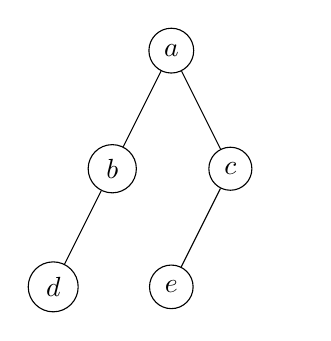
\begin{tikzpicture}[grow=down, sloped]
  \node[draw,fill=white, circle] {$a$}
      child {
          node[draw,fill=white, circle] {$b$}
              child {
                  node[draw,fill=white, circle] {$d$}
                  edge from parent[-]
              }
              child {
                  node[draw=none,fill=none, circle] {}
                  edge from parent[draw=none]
              }
              edge from parent[-]
      } child {
          node[draw,fill=white, circle] {$c$}
              child {
                  node[draw,fill=white, circle] {$e$}
                  edge from parent[-]
              }
              child {
                  node[draw=none,fill=none, circle] {}
                  edge from parent[draw=none]
              }
              edge from parent[-]
      };
  \end{tikzpicture}
  \caption{}
  \label{fig:succ_1}
\end{subfigure}
\begin{subfigure}[t]{0.45\columnwidth}
  \centering
  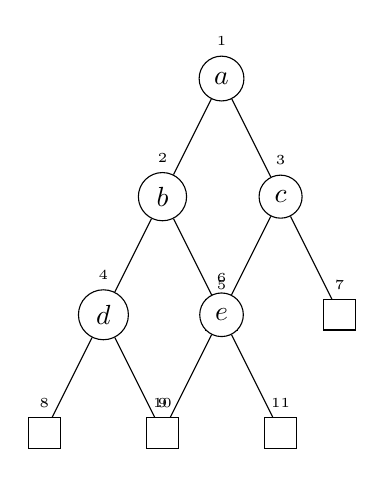
\begin{tikzpicture}[grow=down, sloped]
  \node[draw,fill=white, circle, label={\tiny 1}] {$a$}
      child {
          node[draw,fill=white, circle, label={\tiny 2}] {$b$}
              child {
                  node[draw,fill=white, circle, label={\tiny 4}] {$d$}
                  child {
                      node[draw,fill=none, label={\tiny 8}] {\phantom{a}}
                      edge from parent[-]
                  }
                  child {
                      node[draw,fill=none, label={\tiny 9}] {\phantom{a}}
                      edge from parent[-]
                  }
                  edge from parent[-]
              }
              child {
                  node[draw,fill=none, label={\tiny 5}] {\phantom{a}}
                  edge from parent[-]
              }
              edge from parent[-]
      } child {
          node[draw,fill=white, circle, label={\tiny 3}] {$c$}
              child {
                  node[draw,fill=white, circle, label={\tiny 6}] {$e$}
                  child {
                      node[draw,fill=none, label={\tiny 10}] {\phantom{a}}
                      edge from parent[-]
                  }
                  child {
                      node[draw,fill=none, label={\tiny 11}] {\phantom{a}}
                      edge from parent[-]
                  }
                  edge from parent[-]
              }
              child {
                  node[draw,fill=none, label={\tiny 7}] {\phantom{a}}
                  edge from parent[-]
              }
              edge from parent[-]
      };
  \end{tikzpicture}
  \caption{}
  \label{fig:succ_2}
\end{subfigure}

\caption{The tree $T$ and its succint representation.}
\label{fig:succ_0}
\end{figure}

To construct the succint encoding of $T$, first we have to add empty nodes such
that all the ones that contain data have two children, as shown in
\autoref{fig:succ_2}. Then we number all the nodes from top to bottom and left
to right, obtaining the numbering shown in the picture. That will be the
indexing of our array representation, where every cell contains a bit set to 1
if the corresponding node contains data, or 0 otherwise. The resulting array is
shown in the following table:
%
\begin{center}
  \begin{tabular}{r|c|c|c|c|c|c|c|c|c|c|c}
                   & 1 & 2 & 3 & 4 & 5 & 6 & 7 & 8 & 9 & 10 & 11 \\ \hline
    $B_i$          & 1 & 1 & 1 & 1 & 0 & 1 & 0 & 0 & 0 &  0 &  0 \\
    $Rank_1(B, i)$ & 1 & 2 & 3 & 4 &   & 5 &   &   &   &    &    \\
  \end{tabular}
\end{center}

We can now navigate the succint encoding of the tree using a $Rank_1$ data
structure and the following procedures:
%
\begin{itemize}

  \item $LeftChild(r) = 2 \cdot r$, that given the \emph{rank} $r$ of a node, returns
  the \emph{index} of its left child;

  \item $RightChild(r) = 2 \cdot r + 1$, that given the \emph{rank} $r$ of a node,
  returns the \emph{index} of its right child;

  \item $Parent(i) = \left\lfloor \frac{i}{2} \right\rfloor$, that given the
  \emph{index} $i$ of a node, returns the \emph{rank} of its parent.

\end{itemize}

For example, we can move from the root node $a$ (that has rank $r_a = 1$, since
it's the root node and, then, the first element of the array $B$) to its right
child $c$ with $$i_c = RightChild(r_a) = 2 \cdot r_a + 1 = 3.$$ Then, given the
index $i_c$ we compute its rank with $$r_c = Rank_1(B, i_c) = 3$$ and percolate
the tree once again, this time to its left child $e$, obtaining its index with
$$i_e = LeftChild(r_c) = 2 \cdot r_c + 1 = 6.$$
